\section{Results}
\label{sec:results}
\setlength{\parindent}{10ex}

This section contains the results for each model observed by this work, including results for the regression, classification, and novel grid optimized model.
Each section includes figures representing the metric scores.

\subsection{Regression Results}
The \(R^2\) score for each model can be found in Figure~\ref{fig:r2_barplot_regression}.
The RMSE of each model can be found in Figure~\ref{fig:rmse_barplot_regression}.



\begin{figure}[htp]
    \centering
    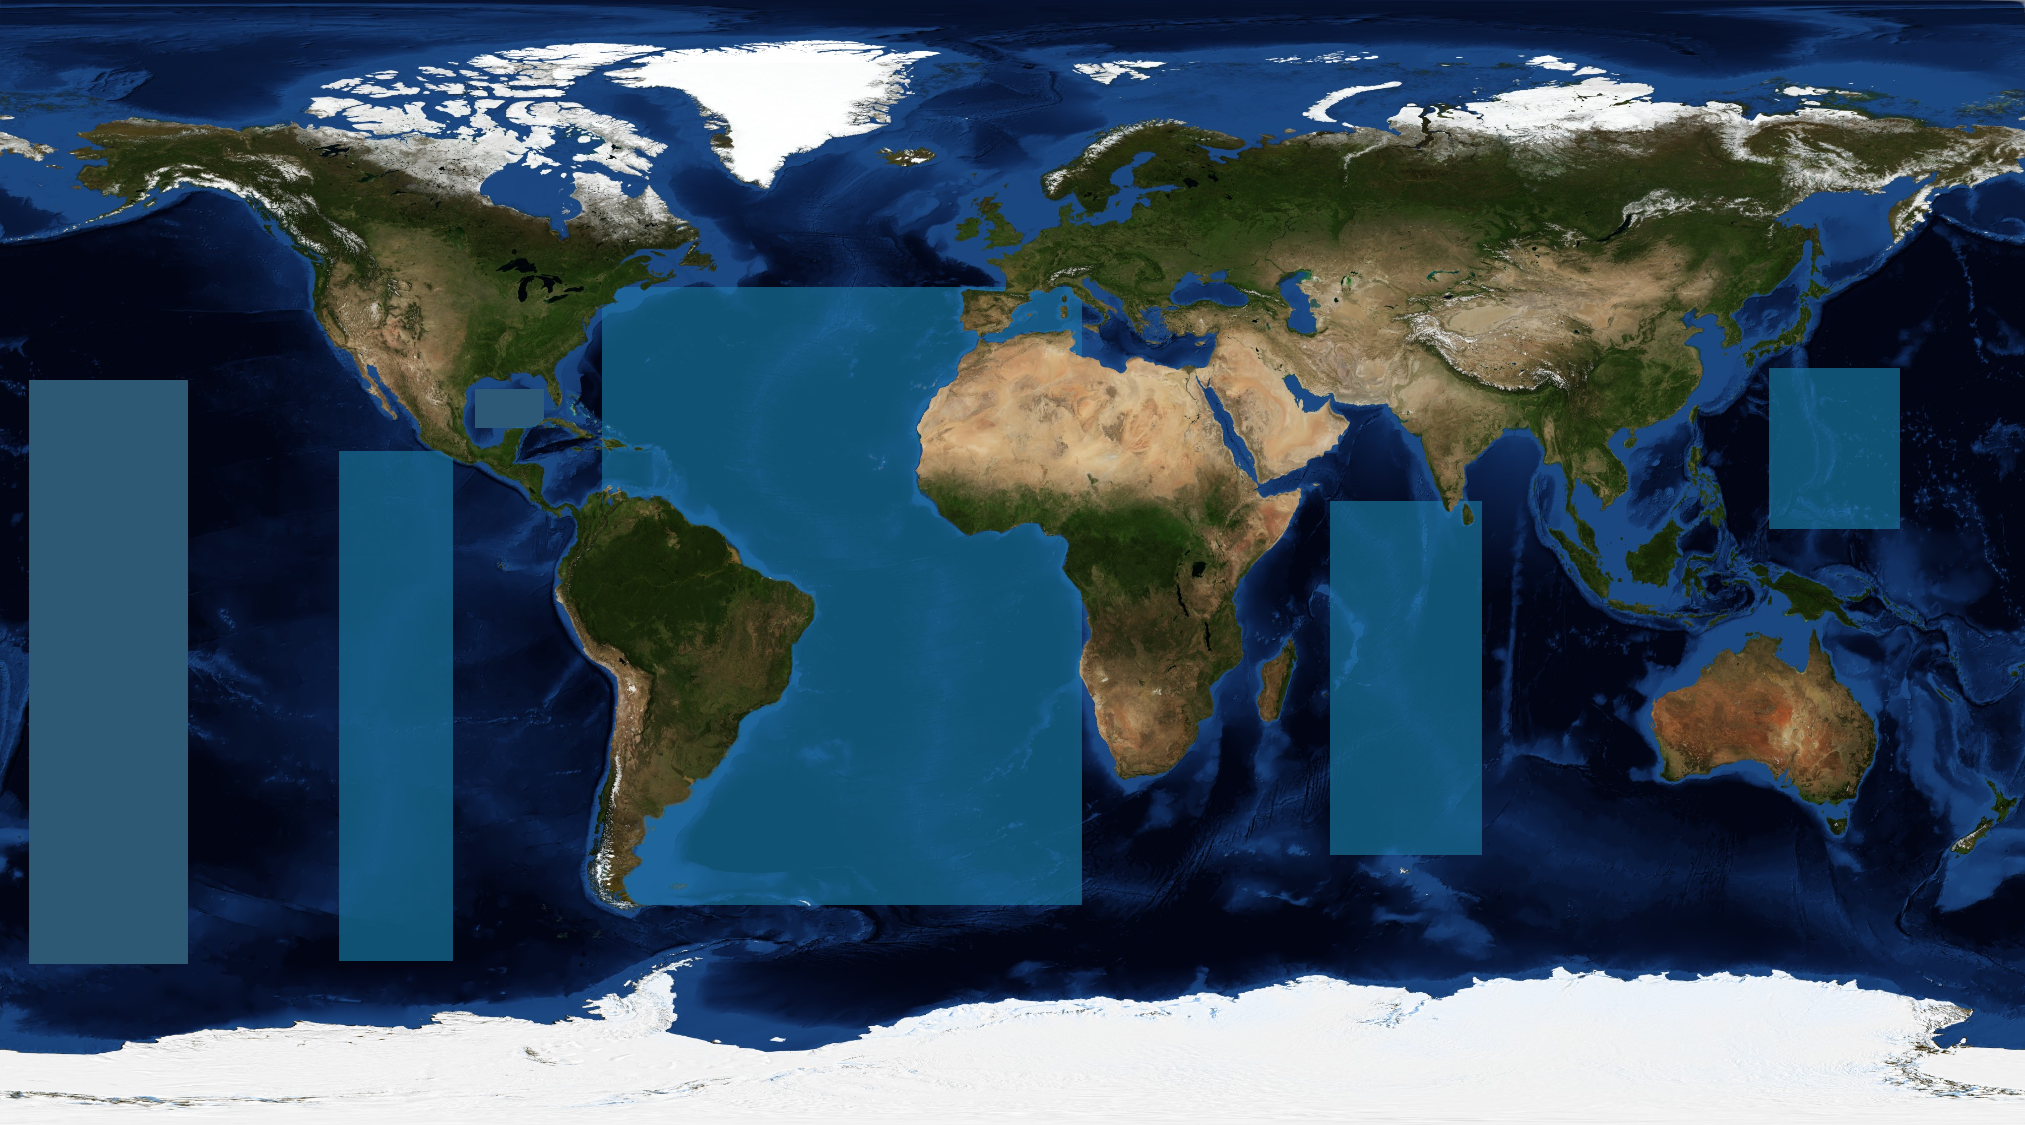
\includegraphics[width=\textwidth]{worldtraininglocal.png}
    \caption{Initial training sets for regression. Testing was performed against the rest of the world.}
    \label{fig:trainset}
\end{figure}

% \begin{table}[htp]
%     \centering
%     \begin{tabular}{|c c c|}
%         \hline
% 		\textbf{Model} & \textbf{\(R^2\)} & \textbf{RMSE} \\
% 		\hline
% 		SVM Regression & 0.841 & 365.23m \\
% 		Naive Bayes & 0.884 & 294.92m \\
%         Linear Regression & 0.885 & 265.43m \\
% 	    \hline
%     \end{tabular}
%     \label{table:REGRESSION_RESULTS}
%     \caption{Regression Results}
% \end{table}

\begin{figure}[htp]
    \centering
    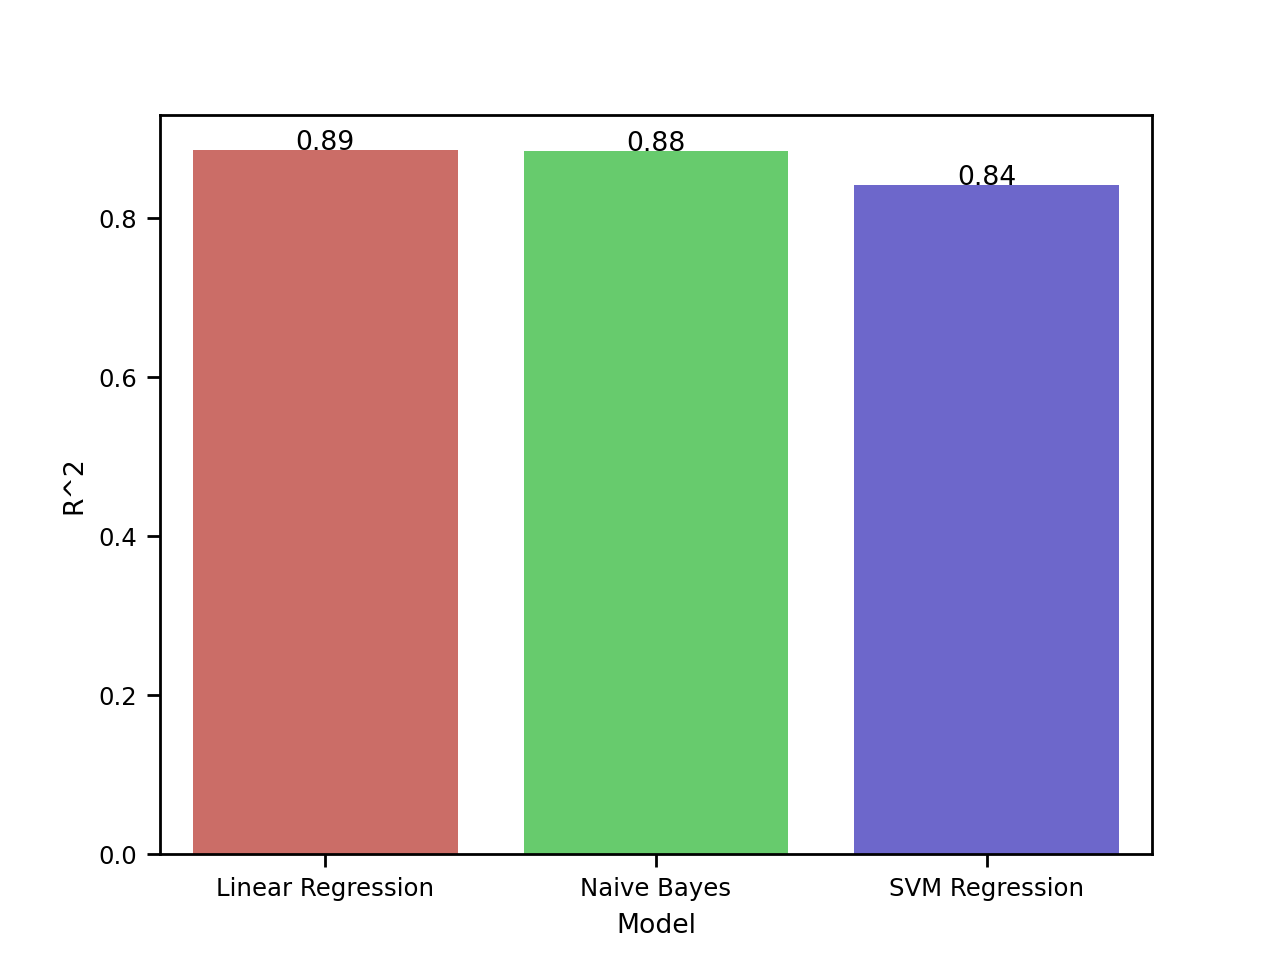
\includegraphics[width=\textwidth]{rsquared_barplot_regression.png}
    \caption{\(R^2\) score for each model. Higher values represent better performing models.}
    \label{fig:r2_barplot_regression}
\end{figure}

\begin{figure}[htp]
    \centering
    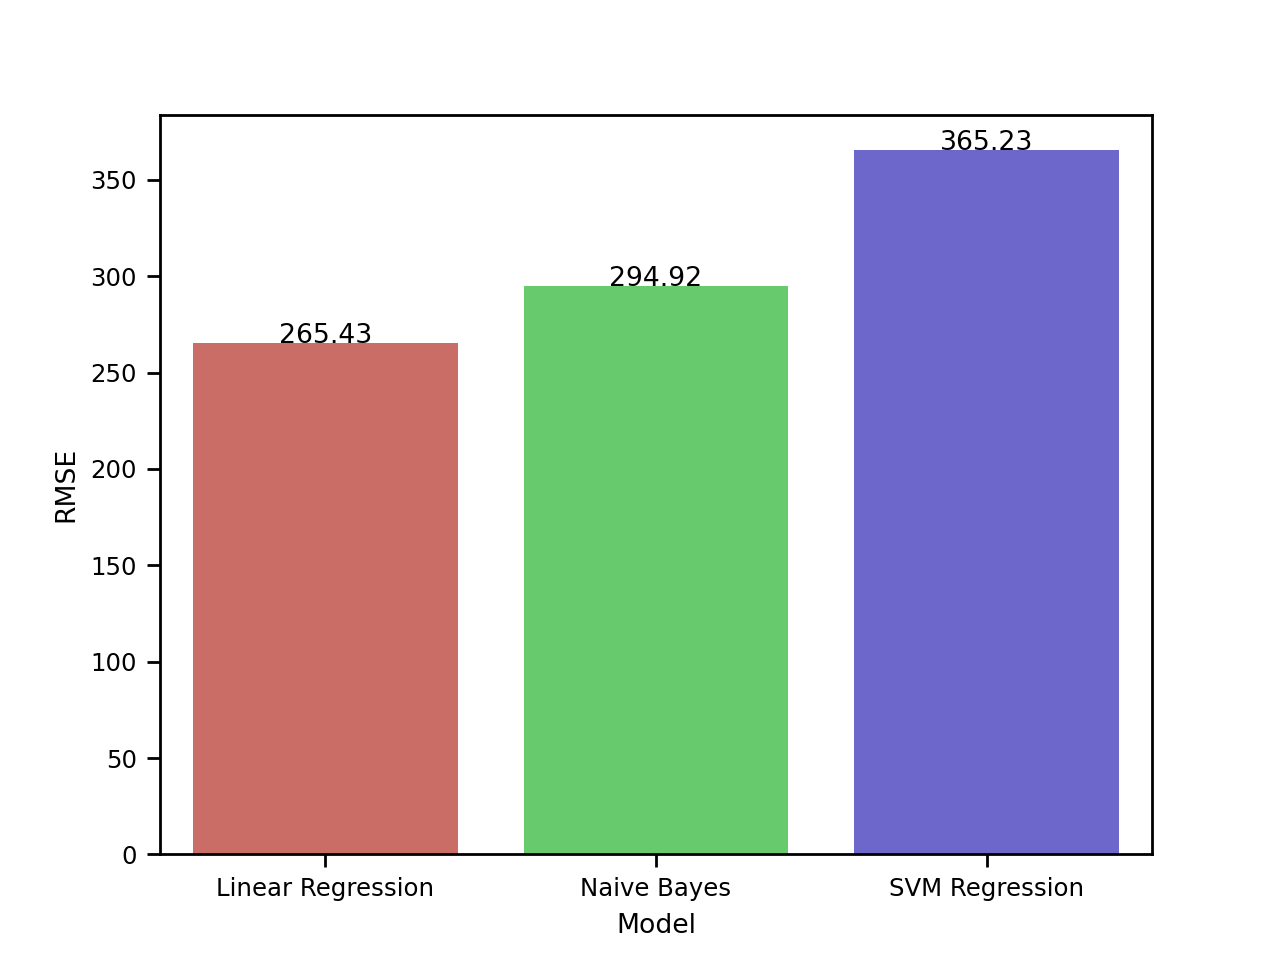
\includegraphics[width=\textwidth]{rmse_bar_regression.png} 
    \caption{RMSE for each model. Lower values represent lower error for a model.}
    \label{fig:rmse_barplot_regression}
\end{figure}

% \subsubsection{Regression Results Discussion}
% \cite{jena2012prediction} achieved a \ac{RMSE} of \~{}175m in their optimized model.
% The linear regression model I fit is 100 meters less accurate than the optimized model used in \cite{jena2012prediction}.
% However, the purpose of the test is not to achieve accurate predictions, but to identify if \ac{ML} models can be viable.
% Therefore, the accuracy of these models is less important than identifying the viability of the models.
% The training data used is essentially predicted bathymetry, but shows that fitting a model to true bathymetry will yield a similar result.
% Analyizing the \(R^2\) score gives evidence of the viability of the model.
% This score suggests that there are underlying relationships in the model that can be used to train a successful model.

\subsection{Classification Results}
\setlength{\parindent}{10ex}
The F1 results for each model can be found in Figure~\ref{fig:f1_barplot_classification}.
The Balanced Accuracy for each model can be found in Figure~\ref{fig:balacc_barplot_classification}.

\par
The Decision Tree classifier performed significantly worse than the other models.
The 47\% balanced accuracy is not usable for predictions.
Potentially, parameter tuning and feature selection could improve this model.

% \begin{table}[htp]
%     \centering
%     \begin{tabular}{|c c c|}
%         \hline
% 		\textbf{Model} & \textbf{Average F1 Score} & \textbf{Mean Balanced Accuracy} \\
% 		\hline
% 		Random Forest & 0.81 & 0.82 \\
%         Bagging & 0.80 & 0.79 \\
%         Decision Tree & 0.44 & 0.47 \\
%         \hline
%     \end{tabular}
%     \label{table:CLASSIFICATION_RESULTS}
%     \caption{Classification Results}
% \end{table}

\begin{figure}[htp]
    \centering
    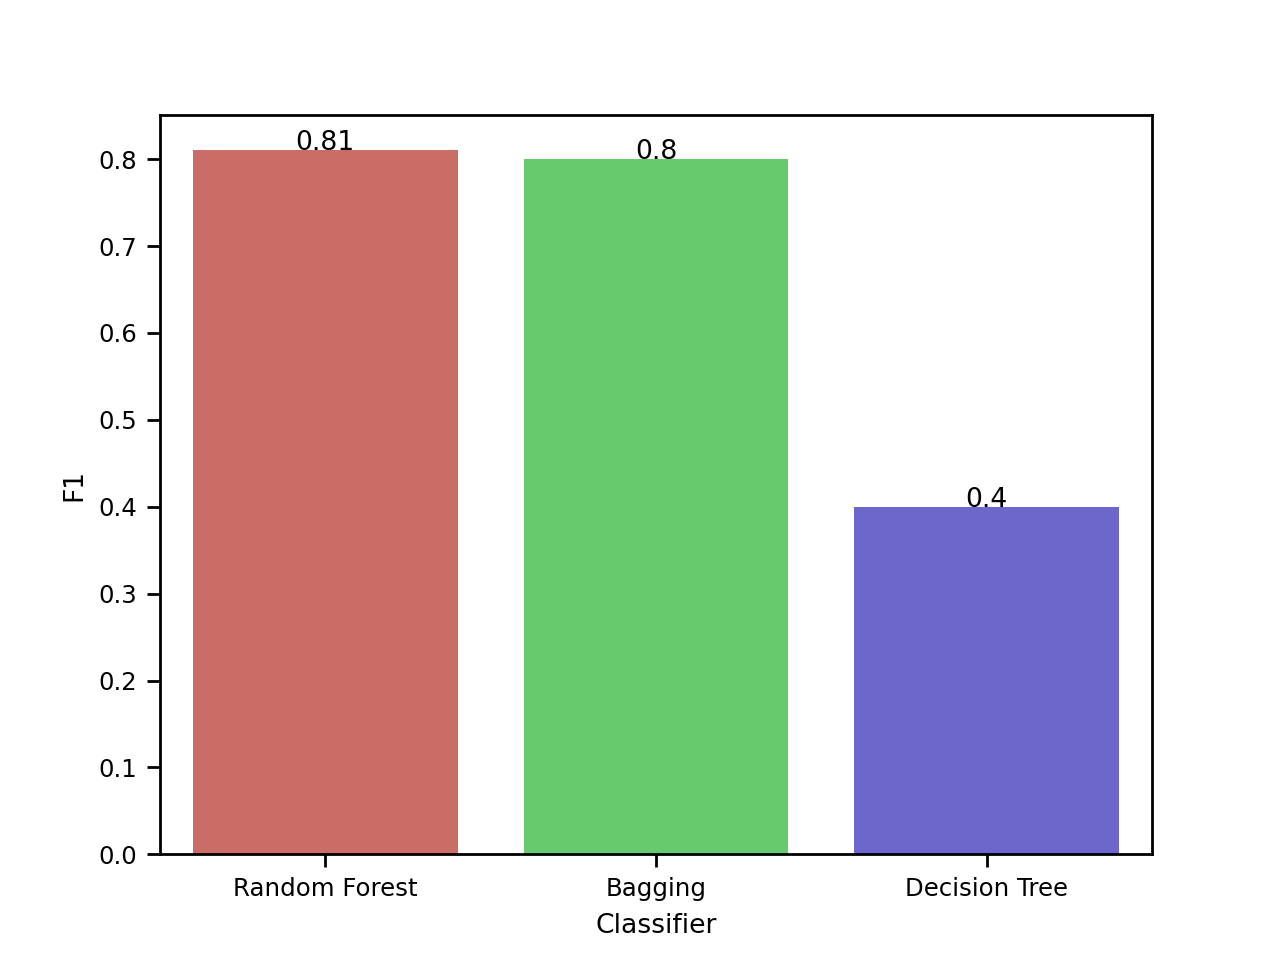
\includegraphics[width=\textwidth]{f1_bar_classification.png}
    \caption{F1 score for each classifier. Higher values represent better precision and recall. From this, we see the Decision Tree does not make useful predictions.}
    \label{fig:f1_barplot_classification}
\end{figure}

\begin{figure}[htp]
    \centering
    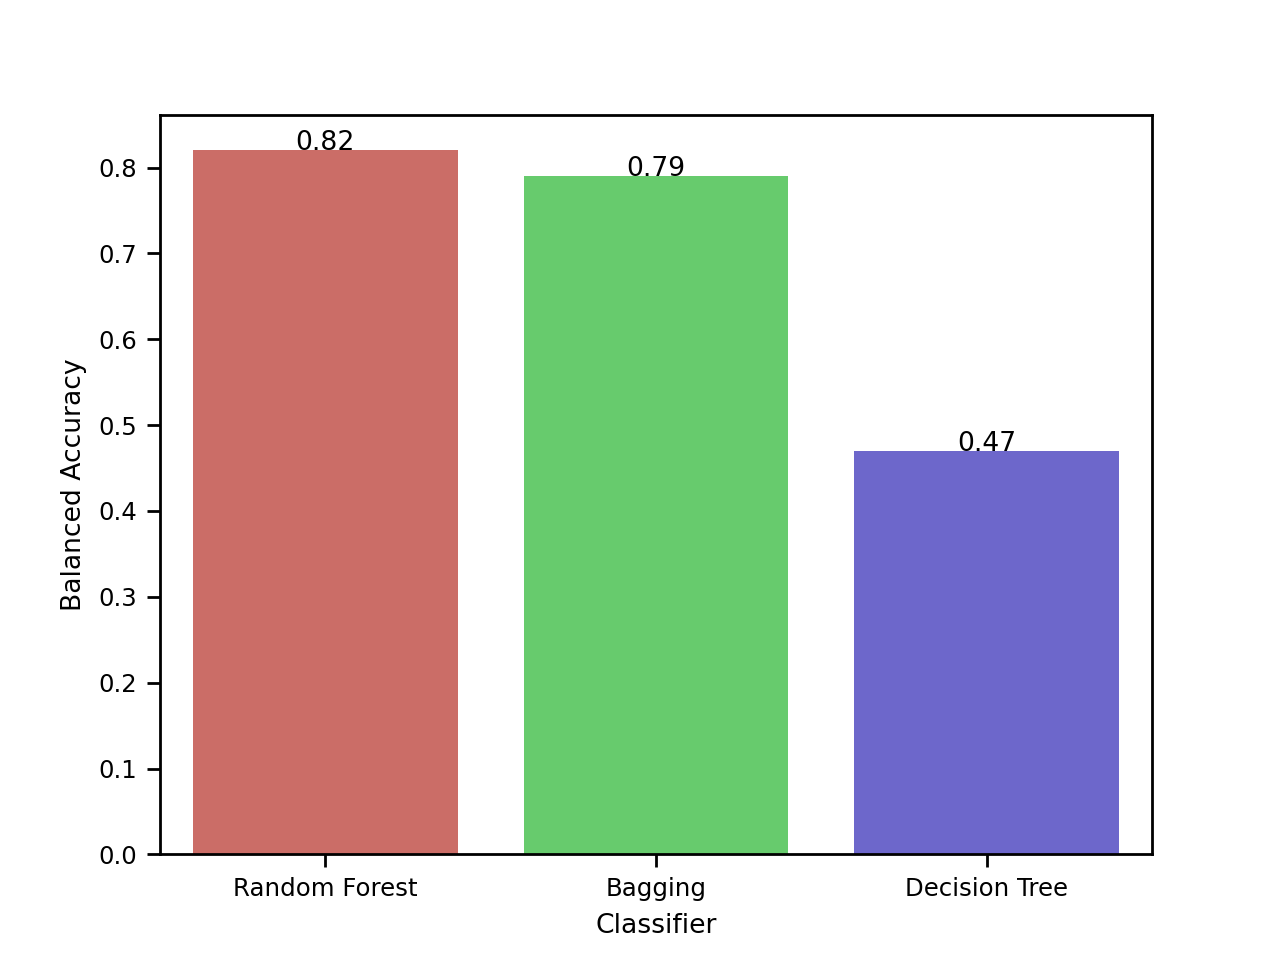
\includegraphics[width=\textwidth]{balacc_bar_classification.png}
    \caption{Balanced accuracy for each classifier. Higher values represent higher accuracy.}
    \label{fig:balacc_barplot_classification}
\end{figure}

\subsection{Grid-Optimization Results}
The Grid Optimized Classifier used the results from Figure~\ref{fig:coveragegrid} as a decision function to select an \textit{optimum} model.
Simply, the classifier checks the location of the prediction for its corresponding grid in Figure~\ref{fig:coveragegrid}.
The model that performed best in that coverage is then used for classification.
This optimum model selection improved the prediction accuracy of the model by several percent.
See Figure~\ref{fig:grid_opt_barplot} for the results of the model.



\newpage

\begin{figure}[htp]
    \centering
    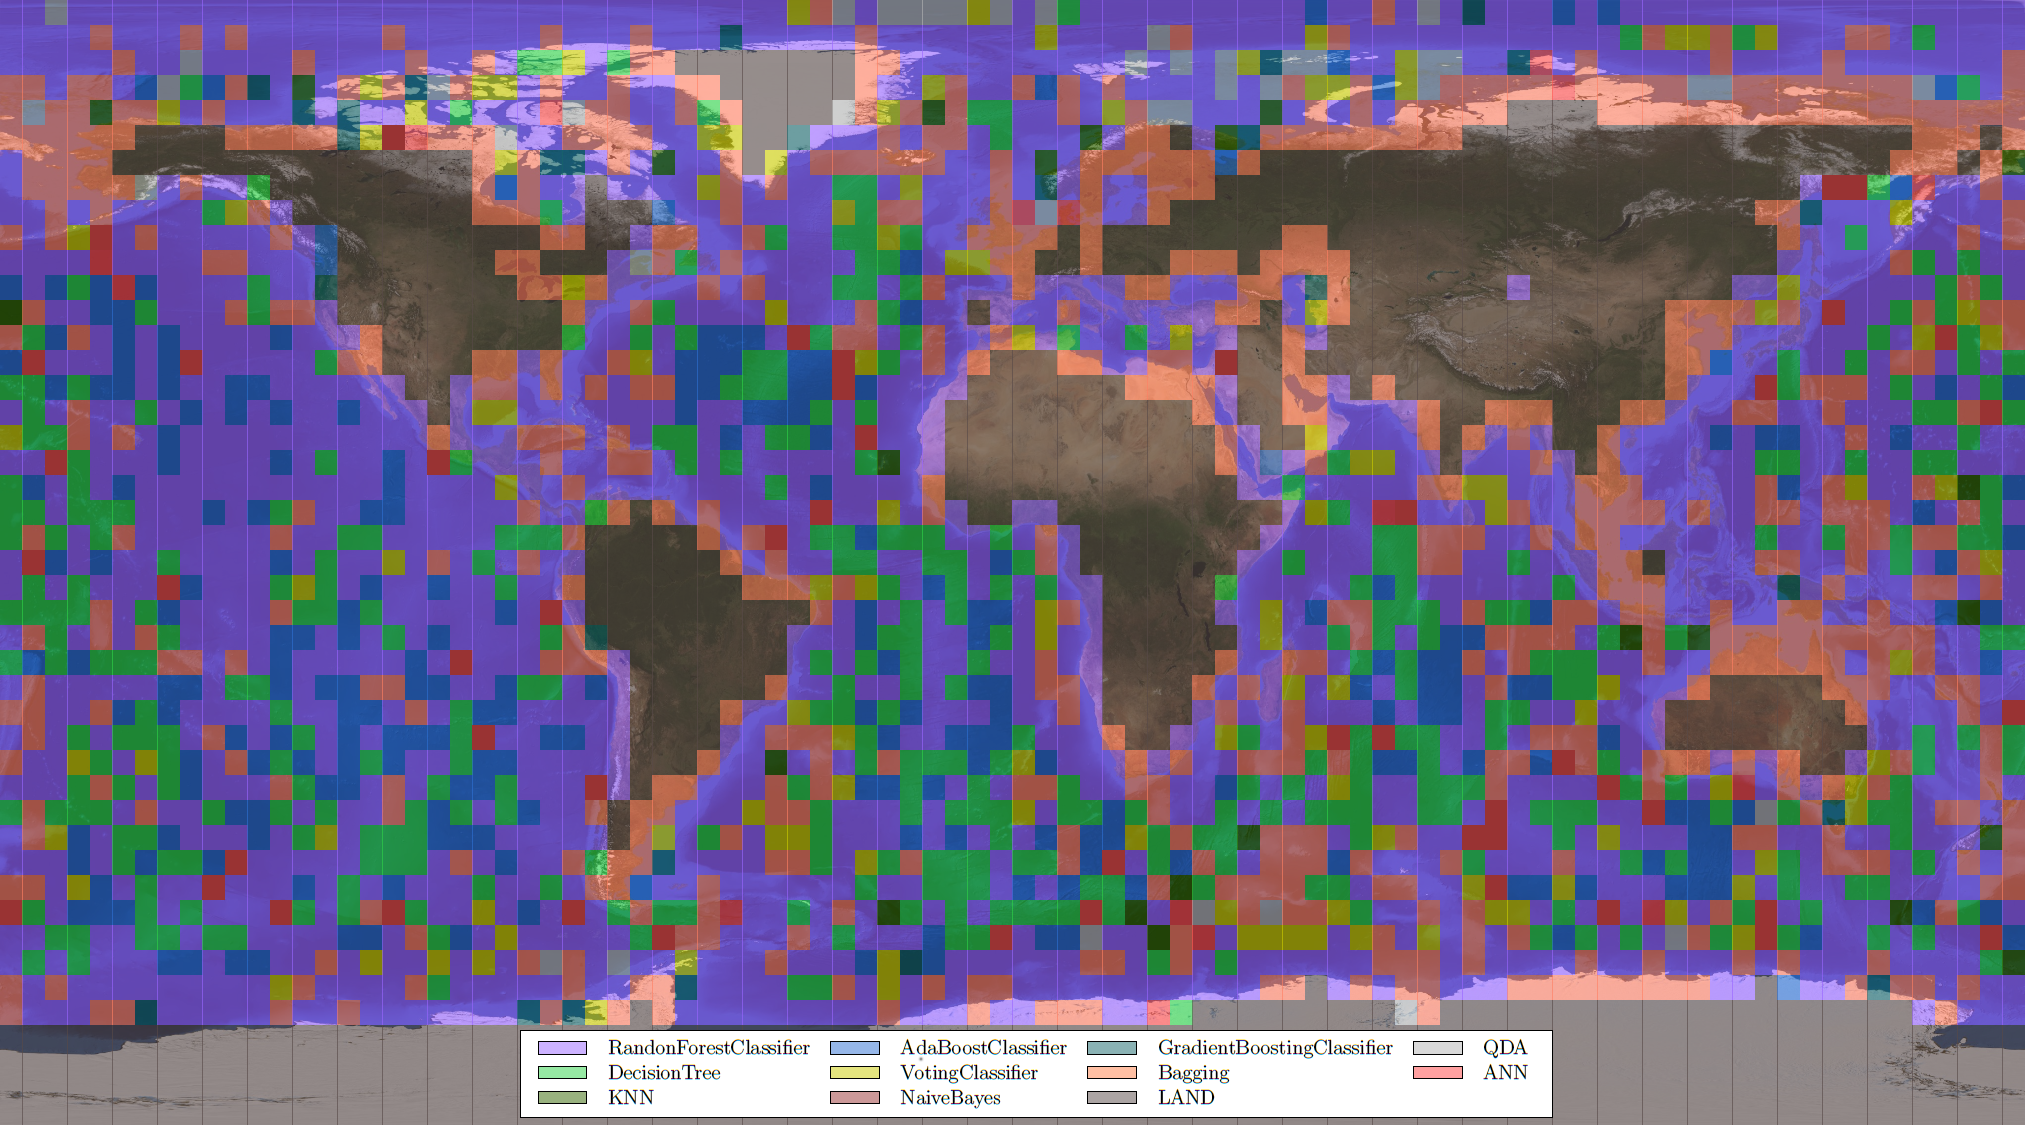
\includegraphics[width=\textwidth]{optgriddraft.png}
    \caption{World Coverages and Successful Models.
    Each square represents a coverage.
    The shaded color represents the model that was most successful in that coverage.}
    \label{fig:coveragegrid}
\end{figure}


\newpage
\begin{figure}[htp]
    \centering
    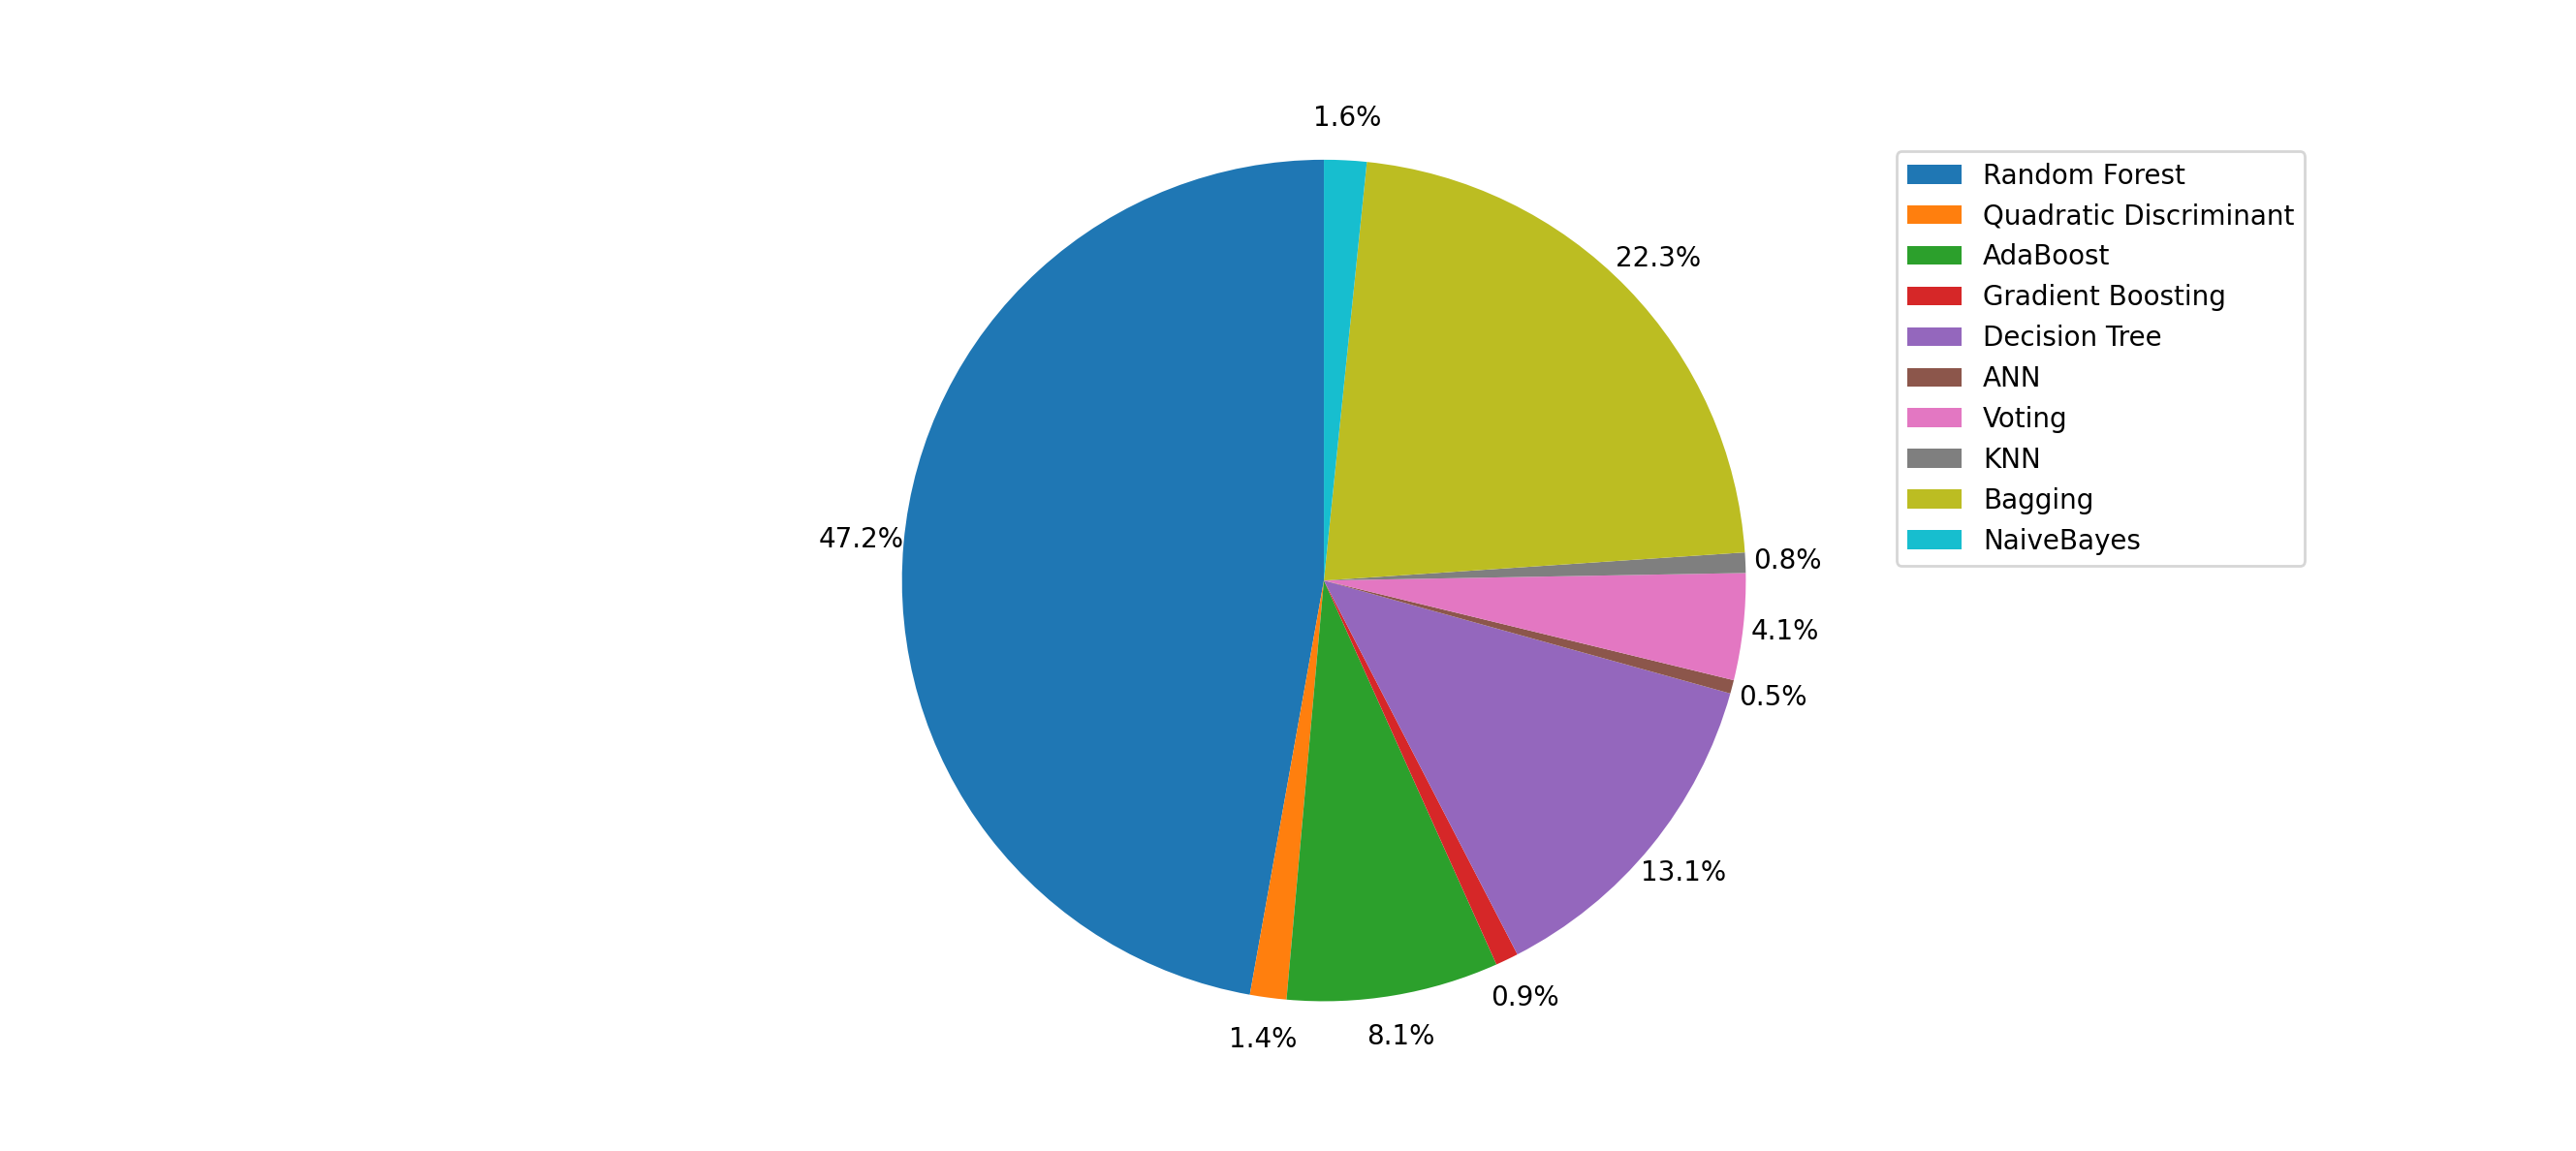
\includegraphics[width=\textwidth]{best_fit_percentage.png}
    \caption{Percentage of coverages where a model was "best fit".}
    \label{fig:pie_best_fit}
\end{figure}

\par
Figure~\ref{fig:coveragegrid} illustrates the coverages where each model performed best.
Figure~\ref{fig:pie_best_fit} shows the percentage that each model was a best fit.
The random forest classifier was the best fit model for a large portion of the oceans.
On the other hand, the Bagging classifier consistently performed well along the coast lines.
The reasons why these classifiers may have performed so well in those areas will be discussed/explained in Section 6.

\newpage
\begin{figure}[htp]
    \centering
    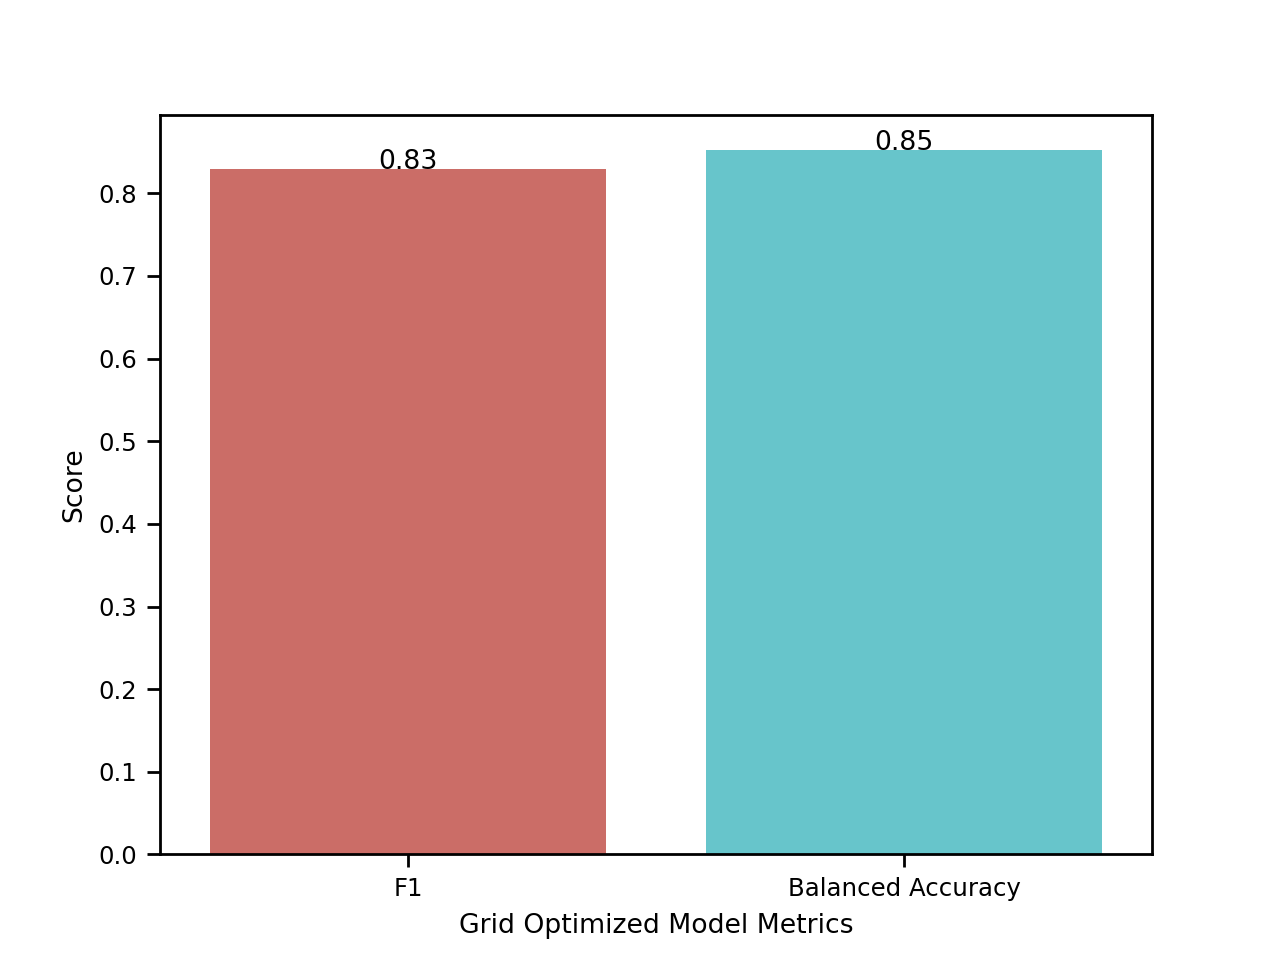
\includegraphics[width=\textwidth]{grid_opt_results.png}
    \caption{Grid Optimized Model results. Higher values represent better performing models.}
    \label{fig:grid_opt_barplot}
\end{figure}
%In this section I am defining what the Grid optimization is and why it matters.
%There may be a better name for this?? Who knows really...

